On page~\pageref{chap:unify} the task description contains a drafted solution called \textsc{SQTL} which is similar to \textsc{SQTL}. This
solution, even if still in work, may not be fast enough to run on small 8 Bit core nodes due to computing power. Additionally, a low-power 
setup does currently not provide enough space for complex query deciphering, at least not in the year 2012. Further development on a 
multifunctional language is the path for the future but a practical solution is not in the reach of \textsc{SQTL}.

Another approach to enable a unified communication is \textsc{wiselib}. The article~\cite{wiselib} is written some of the authors of this
open-source library. By using ``advanced C++ techiques such as templates and inline functions'' algorithms can be used on different nodes
which would not easily be programmed by one source. The problem of applying a gateway and buffering for data on the gateway machine or node itself
is not part of this project. The authors of this paper doubt that C++ is the future of all node algorithms as

\begin{itemize}
    \item C++ will change in the future
    \item nodes will not always be programmable by C++
    \item compilers change
    \item ``\gdir{Πάντα ῥεῖ}'' - \gdir{Ἡράκλειτος}
\end{itemize}

Our approach is more direct and does enable queries due to usage of \textsc{SQL}. 
This logic should be done on the end device, e.g. a Android-powered Smartphone or a 
vanilla i86 machine but can also be part of the gateway's action. 
More complex commands are possible but require additional programming logic on the node's side. We try to 
keep the low-level efforts on the nodes as small as possible to be independent of changing implemenations, standards and dialects.

\cite{Heinzelman00energy-efficientcommunication} describes a system for a homogenous hardware setup so we skip this \textsc{Mit} development as 
our aim is not dependent on specific brands or models of wireless sensor nodes.

\section{Security in Node Communication}

Data sent through wireless nodes may contain protectable data. Note that nodes are used with military and civilian applications. As military does
not release open information about their encryption the civil development concentrates on environment measuring as temperature, pressure and other 
non-important data and health monitoring.\cite{Dispert}
While health data output may not be very interesting to attackers the input side of specific critical health functions.\footnote{Imagine somebody 
just turns off an artificial cardiac clock.}
Our first plans included a security layer based on \textsc{PKCS\#11}. Diagram~\ref{fig:pkcs11} contains a rough setup. \cite{wsnsec} tried to 
use symmetric encryption based on \textsc{AES} which resulted in a 80\% increase in power consumption. A further option was described by 
using the hardware encryption on the Wireless Communication chip on-board but this solution is very specific to specific hardware.

\begin{figure}[h]
   \centering
   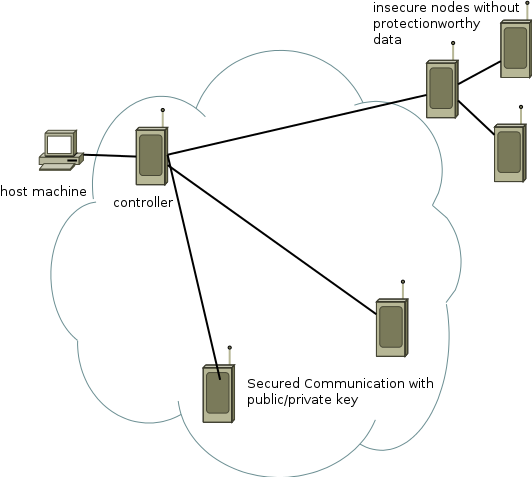
\includegraphics[width=0.6\textwidth]{pic/pkcs11.png}%
   \caption{Former idea with PKCS\#11 enabled communication between nodes}
   \label{pkcs11}%
\end{figure}


\textsc{PKCS\#11}\footnote{public-key cryptography standards} is a collection of standards related to cryptography, especially hardware supported.
In~\cite{PKCS_RSA} the API\footnote{Application Programming Interface} is described over a multitude of sites for the interested reader.
Software tokens are included in every current browser from the Mozilla foundation and all current operating systems(2012) support some means of 
hardware supported cryptography. However, due to licensing and security problems an open implementation is preferred.\footnote{Look at \url{http://www.opensc.org} for further information}

For encryption a public-private key setup could result in a fine-grained setup but there is still no development on the civil side.
The solution we had planned was based on a \(I^2C\) connectable reader for micro-sized smart cards. This would allow a setup where every node
would be addressable by its public key. A sophisticated setup would be possible.\footnote{The reasons for stopping our efforts is on human side. Pretty
bad but not worth mentioning it in this paper.}
